\documentclass[12pt, a4]{article}
\usepackage[english]{babel}
\usepackage[utf8]{inputenc}
\usepackage{fullpage}
\usepackage{listings}
\usepackage{graphicx}
\usepackage{color}

%Syntax highlighting
\definecolor{blue-violet}{rgb}{0.54, 0.17, 0.89}
\definecolor{ao}{rgb}{0.0, 0.5, 0.0}
\definecolor{amaranth}{rgb}{0.9, 0.17, 0.31}
\definecolor{ballblue}{rgb}{0.13, 0.67, 0.8}
\definecolor{onyx}{rgb}{0.06, 0.06, 0.06}


\lstset{
  breaklines=true,                 % automatic line breaking only at whitespace
  captionpos=b,                    % sets the caption-position to bottom
  breakatwhitespace=false,
  keepspaces=true,
  numbers=left,
  numbersep=5pt,
  showspaces=false,
  showstringspaces=false,
  showtabs=false,
  tabsize=4,  
  backgroundcolor=\color{white},   % choose the background color
  commentstyle=\color{ao},    % comment style
  keywordstyle=\color{amaranth},    % keyword style
  stringstyle=\color{blue-violet},    % string literal style
  numberstyle=\tiny\color{ballblue},	   % number style
  basicstyle=\ttfamily\footnotesize\color{onyx} % size of fonts used for the code
}


%Document Header
\title{\textbf{Department of CSE\\SSN College of Engineering}}
\author{\textbf{Vishakan Subramanian - 18 5001 196 - Semester VI}}
\date{13 April 2021}

\begin{document}
\maketitle
\hrule
\section*{\center{UCS 1611 - Internet Programming Lab}}
\hrule
\bigskip

%Assignment Details
\subsection*{\center{\textbf{Exercise 6: Autocomplete Feature Using AJAX}}}
\subsection*{\flushleft{Learning Objective:}}
\begin{flushleft}

\begin{enumerate}
\item Develop an AJAX program that implements the Autocomplete feature for filling the country names.
\item For Example, when N is entered all the names of the country starting with “N” should be listed in drop-down list for user’s easy selection.
\item When “Na” is typed only “Namibia” and “Nauru” should be listed for selection.
\item Use Servlet for server side scripting. 
\item Use MySQL database to store the countries names. 
\end{enumerate}
 
\end{flushleft}

%Code
\newpage
\subsection*{\flushleft{Code - Search Page HTML:}}
\begin{flushleft}
\lstinputlisting[language = HTML]{autocomplete/index.html}
\end{flushleft}

\newpage
\subsection*{\flushleft{Code - CSS Code:}}
\begin{flushleft}
\lstinputlisting[language = HTML]{autocomplete/styles.css}
\end{flushleft}

\newpage
\subsection*{\flushleft{Code - Search Page JavaScript:}}
\begin{flushleft}
\lstinputlisting[language = Java]{autocomplete/scripts/index.js}
\end{flushleft}

\newpage
\subsection*{\flushleft{Code - Web XML:}}
\begin{flushleft}
\lstinputlisting[language = XML]{autocomplete/WEB-INF/web.xml}
\end{flushleft}

\newpage
\subsection*{\flushleft{Code - FetchServlet:}}
\begin{flushleft}
\lstinputlisting[language = Java]{autocomplete/FetchServlet.java}
\end{flushleft}

\newpage
\subsection*{\flushleft{Code - SQL Script:}}
\begin{flushleft}
\lstinputlisting[language = SQL]{autocomplete/scripts/script.sql}
\end{flushleft}

%Output
\newpage
\subsection*{\flushleft{Output - Search Page:}}
\begin{figure}[h]
\centering
\caption{Browser Output: Search Page.}
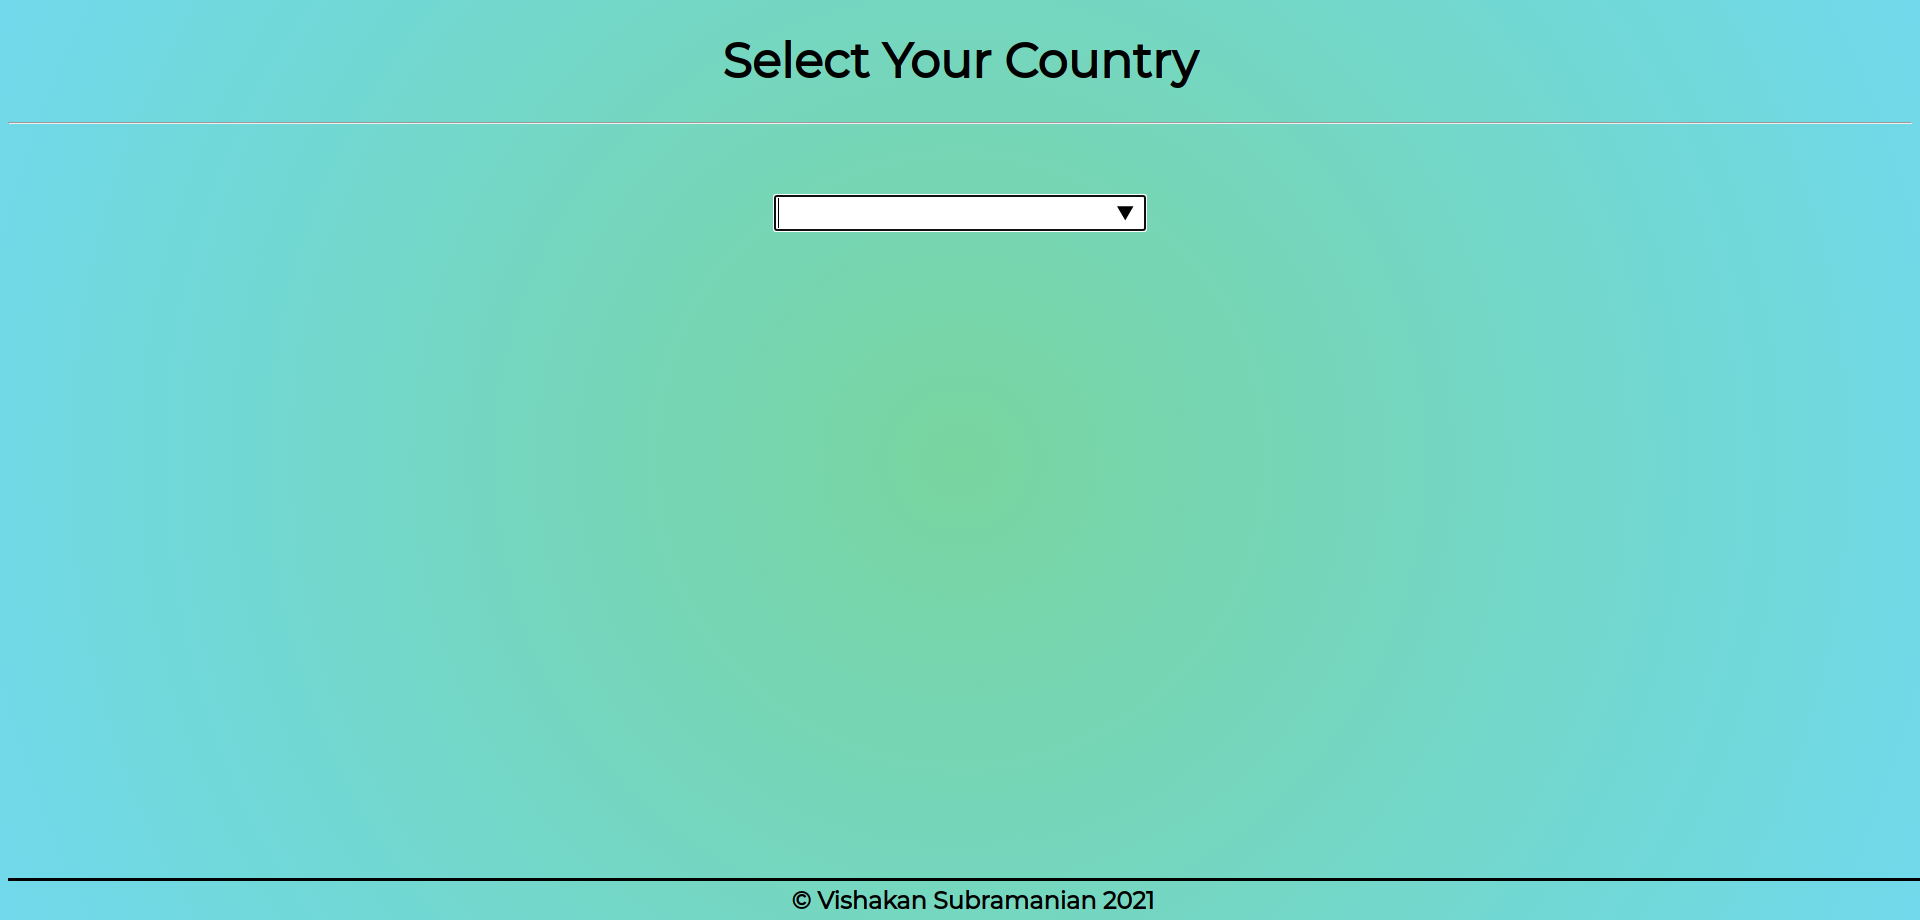
\includegraphics[height=15cm, width=18cm]{Output/Autocomplete1.png}
\end{figure}

\newpage
\subsection*{\flushleft{Output - Search (I) Page:}}
\begin{figure}[h]
\centering
\caption{Browser Output: Search (I) Page.}
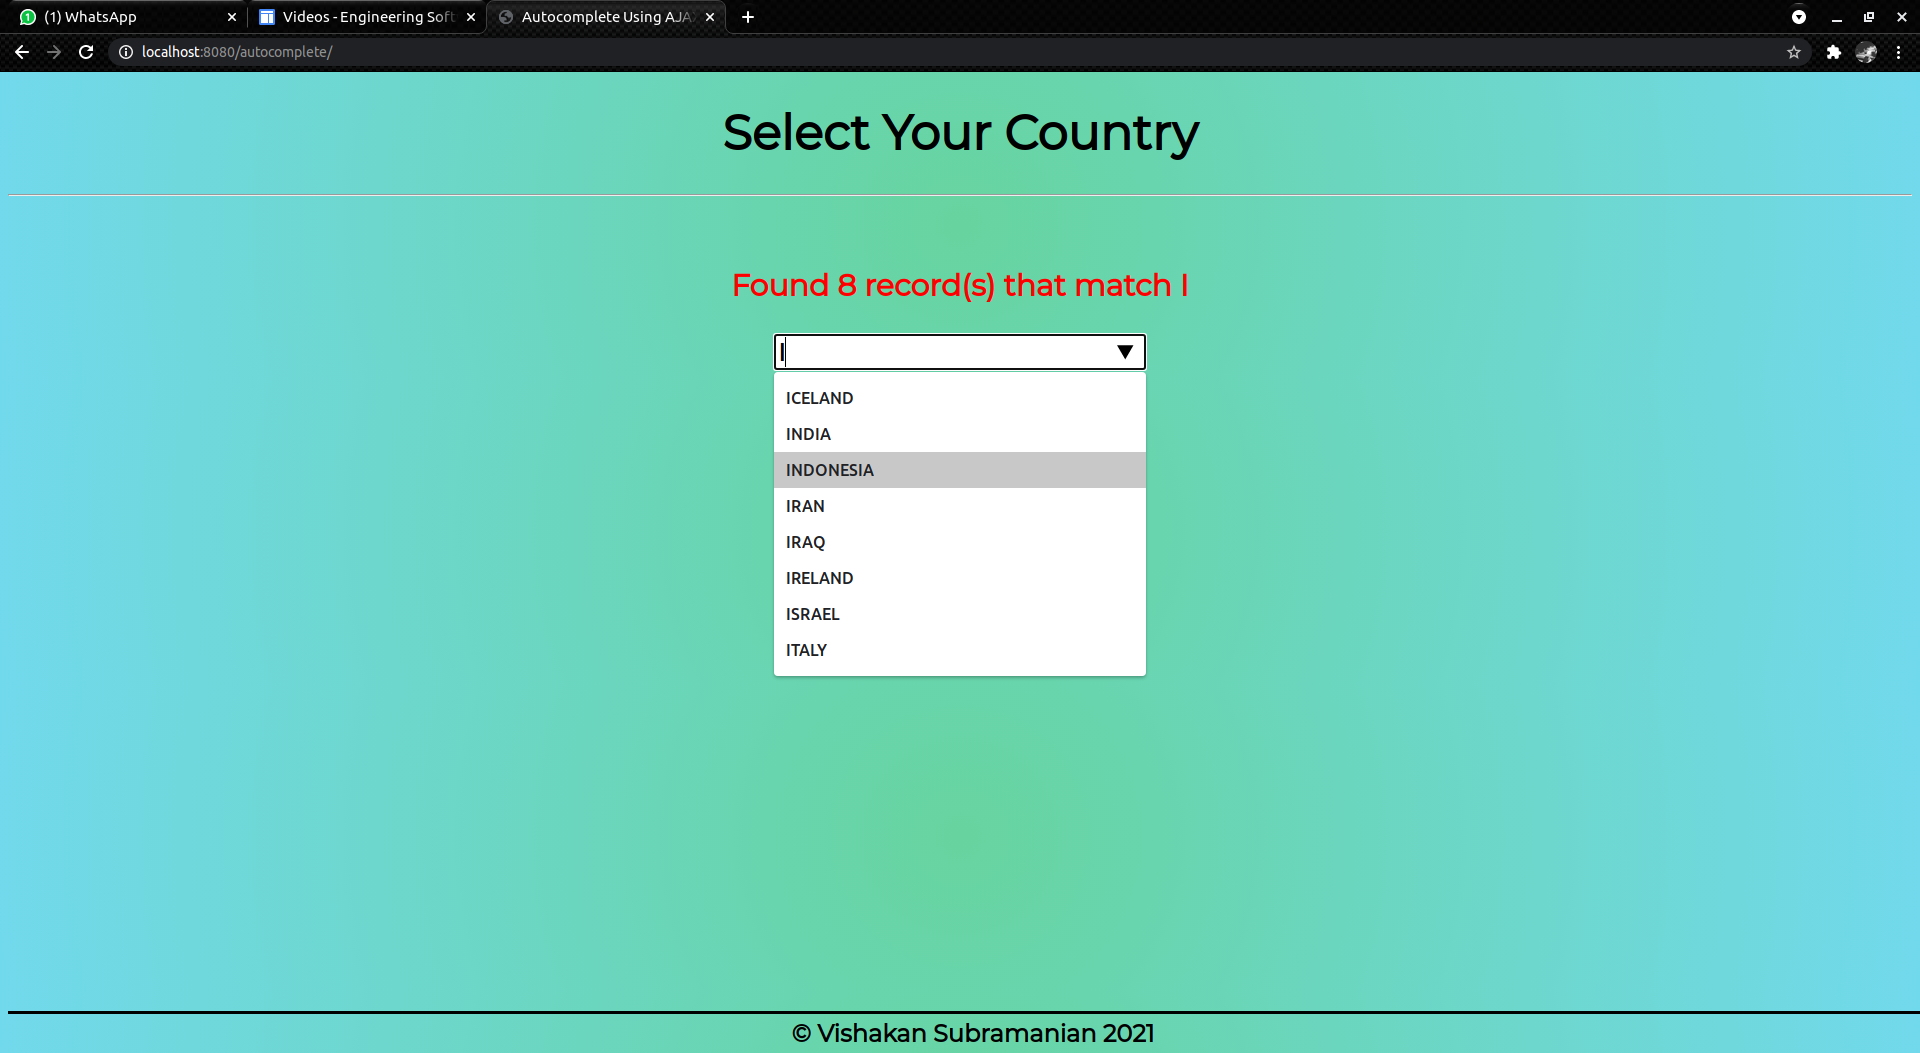
\includegraphics[height=12cm, width=18cm]{Output/Autocomplete2.png}
\end{figure}

\newpage
\subsection*{\flushleft{Output - Search (IN) Page:}}
\begin{figure}[h]
\centering
\caption{Browser Output: Search (IN) Page.}
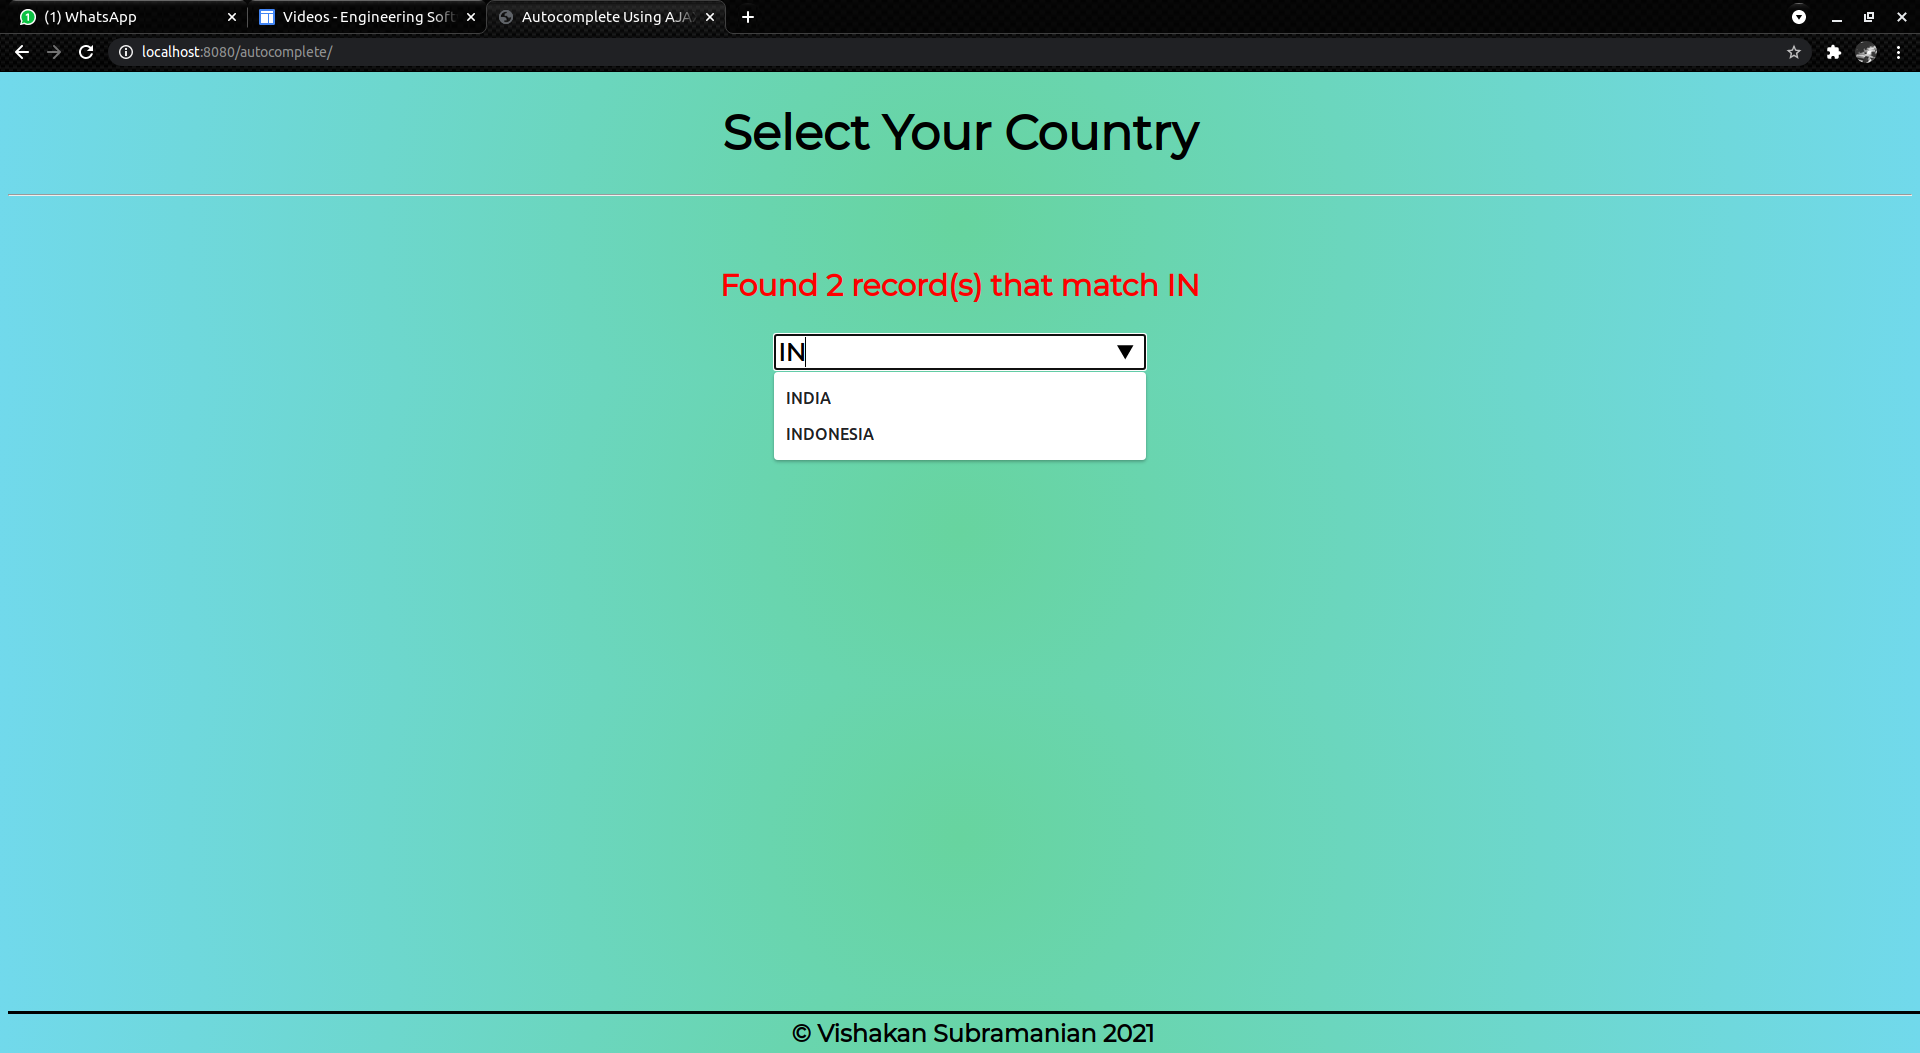
\includegraphics[height=12cm, width=18cm]{Output/Autocomplete3.png}
\end{figure}

\newpage
\subsection*{\flushleft{Output - Search (INDIA) Page:}}
\begin{figure}[h]
\centering
\caption{Browser Output: Search (INDIA).}
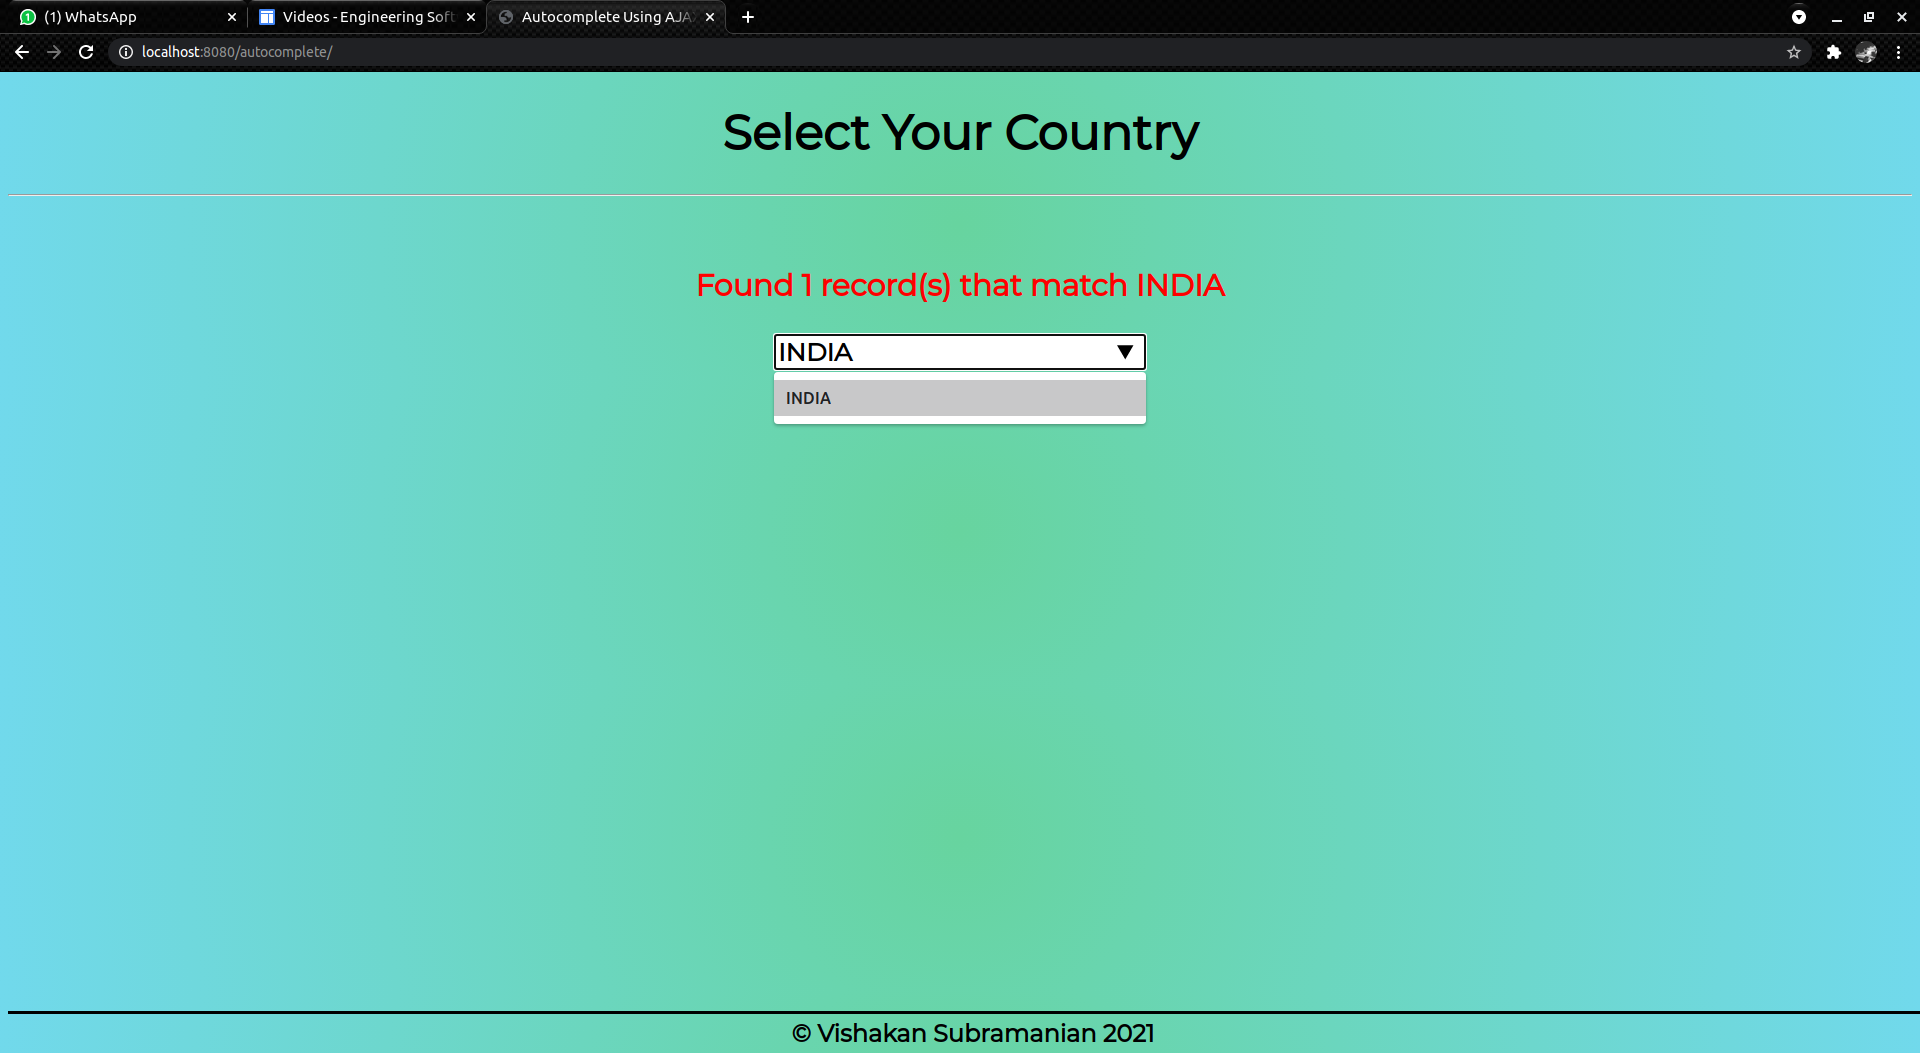
\includegraphics[height=12cm, width=18cm]{Output/Autocomplete4.png}
\end{figure}

\newpage
\subsection*{\flushleft{Output - SQL Table:}}
\begin{figure}[h]
\centering
\caption{Browser Output: SQLTable.}
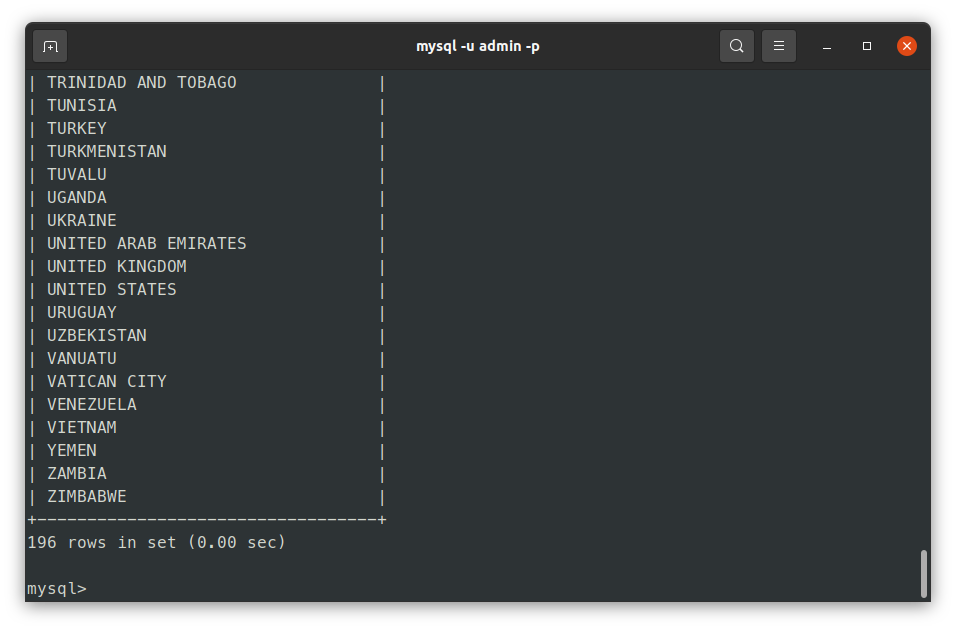
\includegraphics[height=12cm, width=18cm]{Output/SQLTable.png}
\end{figure}

%Learning Outcome
\newpage
\subsection*{\flushleft{Learning Outcome:}}
\begin{itemize}

\item From the experiment, I learnt to implement \textbf{Java Servlets}.
\item I learnt how to serve an XML document from the server-side dynamically using Java Servlets.
\item I was able to integrate a MySQL database to my Java Servlet program using JDBC connector.
\item I was able to pass a GET method call from my client-side using JavaScript with the use of an \textbf{XHTTPRequest Object}.
\item I understood the basic working and process of an \textbf{AJAX request and retrieval}.
\item I was able to parse the XML document retrieved using AJAX with the help of JavaScript DOM methods like getElementsByTagName() and getElementById().
\item I modified my HTML document dynamically with JavaScript and was able to add the relevant countries as per the user's query string by creating \textbf{Node objects} and appending them as a child to a root element in the HTML page, and set it's value attribute using setAttribute() method.
\item I was able to remove all child nodes of the root element using removeChild() method.
\item I learnt to query SQL using \textbf{Regular Expressions}.
\item I understood the importance of closing SQL connections in Java once the records had been retrieved. Failure to close the connections leads to too many open connections if the user changes his/her query frequently and the program failing to work in the front-end side due to that.
\item I was able to implement a working \textbf{Autocomplete Feature} using AJAX.


\end{itemize}

\end{document}
